\documentclass[10pt]{article}
\usepackage[utf8]{inputenc}
\usepackage{url}
\usepackage{hyperref}
\usepackage{amsmath}
\usepackage{amsfonts}
\usepackage{amssymb}
\usepackage{graphicx}
\graphicspath{ {./images/} }
\usepackage{float}
\usepackage{lipsum}
\usepackage{sectsty}
\sectionfont{\centering}
\usepackage{multicol}
\usepackage{xcolor}
\usepackage{natbib}
\usepackage{graphicx}
\usepackage{listings}
\usepackage{xcolor}
\usepackage[font=small]{caption}
\addtolength{\abovecaptionskip}{-3mm}
\addtolength{\textfloatsep}{-5mm}
\setlength\columnsep{20pt}

\usepackage[a4paper,left=1.50cm, right=1.50cm, top=2cm, bottom=3cm]{geometry}


\author{}

\title{\Large{Design and Analysis of Algorithms Assignment}}

\begin{document}
	
	\begin{center}
		{\Large \textbf{Design and Analysis of Algorithms Assignment}}\\
		\vspace{1em}
		{\large Department of Information Technology,}\\
		\vspace{1em}
		\large{Indian Institute of Information Technology, Allahabad 211015, India}\\
		\vspace{1em}
		\large{Abhinav(IIT2019098), Harsh Sharma(IIT2019097), Nitesh Rawat(IIT2019099)}
		\vspace{2.5em}
		
	\end{center}
	
\begin{multicols*}{2}

    \textbf{\emph{{Abstract}: Fractional Knapsack, Given weights and values of n items, we need to put these items in a knapsack of capacity W to get the maximum total value in the knapsack.}}\\
	
	\textbf{\emph{{Index Terms}: Arrays, Greedy, Implementation\\}}


\section*{INTRODUCTION}

Given weights and values of n items, we need to put these items in a knapsack of capacity W to get the maximum total value in the knapsack. There are different cases of knapsack, like in the 0-1 Knapsack problem, we are not allowed to break items. We either take the whole item or don’t take it. In our case (Fractional Knapsack), we can break items for maximizing the total value of knapsack. This problem in which we can break an item is also called the fractional knapsack problem. 

\paragraph{Greedy Algorithm}
Greedy is an algorithmic paradigm that builds up a solution piece by piece, always choosing the next piece that offers the most obvious and immediate benefit. So the problems where choosing locally optimal also leads to global solution are best fit for Greedy.It is a simple, intuitive algorithm that is used in optimization problems. The algorithm makes the optimal choice at each step as it attempts to find the overall optimal way to solve the entire problem. Greedy algorithms are quite successful in some problems, such as Huffman encoding which is used to compress data, or Dijkstra's algorithm, which is used to find the shortest path through a graph.
However, in many problems, a greedy strategy does not produce an optimal solution such as 0/1 knapsack.
But, if we consider the case of fractional knapsack, greedy approach works well.

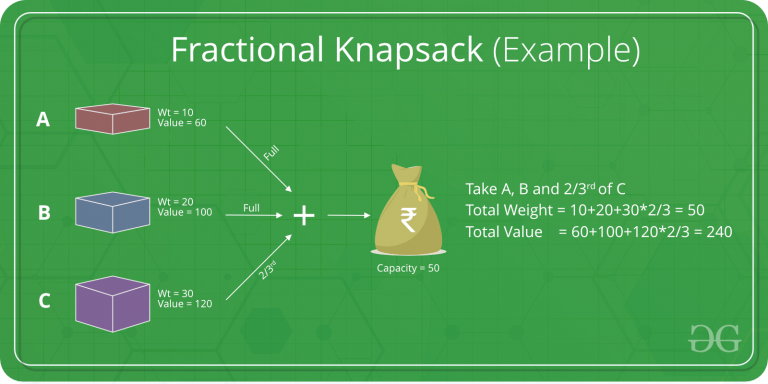
\includegraphics[width=\columnwidth, height=8cm]{Fractional Knapsack.png}\begin{center}\textbf{Figure 1:} Greedy Algorithm (Example)\end{center}


\paragraph{Advantages of Greedy Apporach:}
The Greedy Algorithm generally has following mentioned advantages over Brute Force Algorithms.\\\\
\textbf{Time Efficiency: } This approach generally reduces the running time of the algorithm because the running time of algorithm based on Brute Force is in general high order in nature. But when we are using the approach based on greedy, this running time generally decreases because we don't have to calculate for every possible way, we just pick of best solution at each step. \\
\textbf{Space Efficiency: } The greedy approach algo doesn't need much extra space to solve the problem, it takes constant space other than the input. \\
\\\\\\\\This report further contains:
\begin{itemize}
\item 	Algorithm  Designs
\item 	Algorithm  Analysis
\item 	Experimental Study and Profiling
\item 	Conclusion
\item 	References
\item 	Appendix
\end{itemize}

\section*{ALGORITHM DESIGN}
A general problem based on the Greedy Algorithm.

\paragraph{Algorithmic Steps:}

Let total items be n, the knapsack capacity be W. and let us store the items weight and profit in array of pairs, say pair<double,double>ar[n], It w $\geq$ total weight of the items, we take all the items, otherwise we first choose those items whose profit/weight is maximum, we keep on doing it until the current's item weight is more than the capacity of bag remaining, then finally we take a part of the last item remaining (a fraction of it).
\begin{enumerate}

\item	Input the number n, and w (total no. of items and capacity of the knapsack).
\item	Input the weight and cost of each item in the next n lines.
\item   Sort the items based on their profit to weight ratio.
\item	Declare two variable currentWeight and currentProfit, and initialize them with 0.
\item	Run a loop for each item, if ar[i].second (weight of ith item) + the current weight is less than W, we take the whole item add ar[i].second (profit) to our current profit and increase current weight by ar[i].second, otherwise we take a part of the ith item, (w - currentweight)/(ar[i].second) of the last item, add add ar[i].first * ((w-total weight)/(ar[i].second)) to our currentprofit, and make total weight = w.
\item	Finally, our answer is stored in current profit, we print that.
\\\
\end{enumerate}

\lstset { %
    language=C++,
    backgroundcolor=\color{black!5},
    basicstyle=\footnotesize,
}

\begin{lstlisting}

Int:
Function main()
    input n,w
    pair {double,double} arr[n]
    input arr
    current_weight = 0, current_profit = 0
    sort(arr,arr+n) 
    //based to value of arr[i].first/arr[i].second
    for i = 0 to n:
        if current_weight + arr[i].second <= w:
            current_weight += arr[i].second
            current_profit += arr[i].first
        else:
            current_profit += arr[i].first * 
                (w - current_weight)/arr[i].second
            current_weight=w
    print (current_profit)

\end{lstlisting}
    

	
\section*{ALGORITHM ANALYSIS} 
	
APRIORI ANALYSIS: Let T(n) and S(n) is the time and space respectively with input parameters defined above.(Here n is the length of the string)

\paragraph{TIME COMPLEXITY DERIVATION:} It is quite easy to see that we just sort the items based of their profit/weight, which takes nlogn time. then run a single linear loop to calculate our optimal profit, which take linear time. So our total time compleixty will be O(nlog(n)).
\paragraph{DIFFERENT CASES:} Now let us consider our algorithm in different 
scenarios.\\\\\textbf{BEST CASE/AVERAGE CASE/WORST CASE:} The time and space complexity of our approach in all the three cases is same , i.e, Time Complexity is  O(nlog(n)),in any case. Space complexity is the O(n) in any case, for storing the values.

\section*{PROFILING}

So, after the above analysis, let us have the glimpse of space and time graph about the approach.

\paragraph{TIME ANALYSIS:}Following is the graph representing the time complexity of the algorithm.\\\\\\
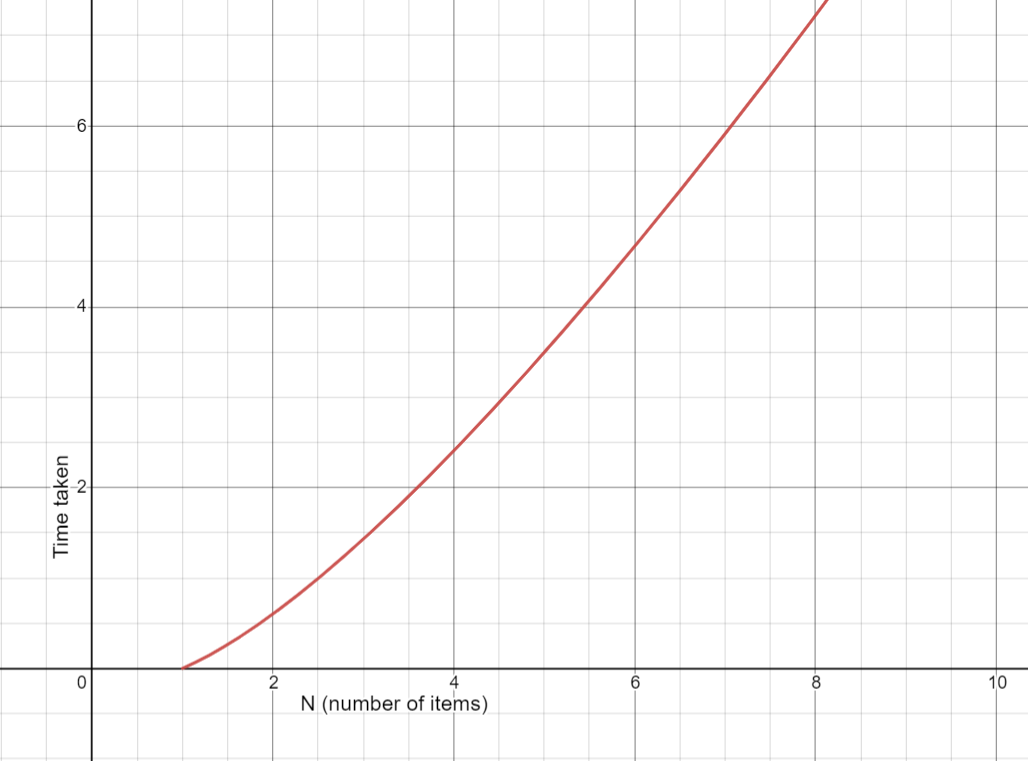
\includegraphics[width=\columnwidth, height=8cm]{Time Complexity.png}\begin{center}\textbf{Figure 2:} Time Complexity Graph\end{center}By the experimental analysis, we found that the more is the value of n, the more time it takes.

\paragraph{SPACE ANALYSIS:}Following is the graph representing the space complexity of the algorithm.\\\\\\
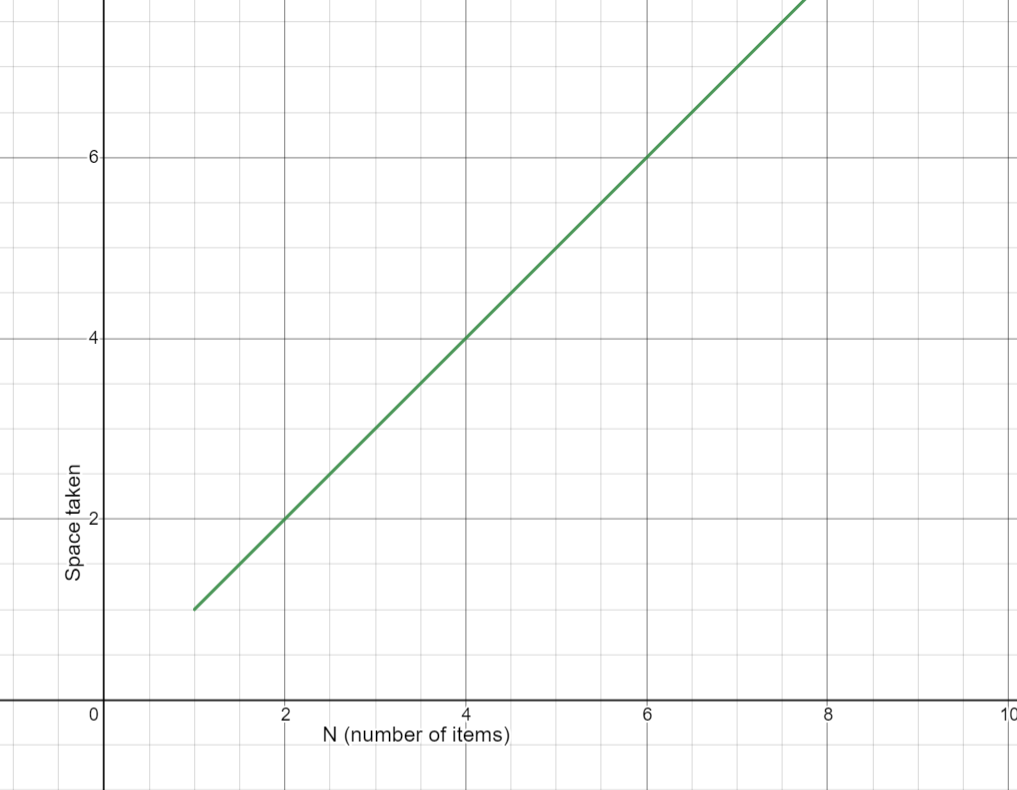
\includegraphics[width=\columnwidth, height=8cm]{Space Complexity.png}\begin{center}\textbf{Figure 3:} Space Complexity Graph\end{center}By the experimental analysis, we found that the more is the value of n, the more space it takes.

\section*{APPLICATIONS}
Greedy Algorithms works step-by-step, and always chooses the steps which provide immediate profit/benefit. It chooses the “locally optimal solution”, without thinking about future consequences. Greedy algorithms may not always lead to the optimal global solution, because it does not consider the entire data. The choice made by the greedy approach does not consider the future data and choices. Some of the applications of the Greedy Approach are:

\begin{enumerate}
\item \textbf{Djikstra Shortest Path Algorithm :} Given a graph and a source vertex in the graph, we find shortest paths from source to all vertices in the given graph by updating the distance of the nodes from source node and from a multiset at each iteration.
\item  \textbf{Kruskal’s Minimum Spanning Tree :} We find a spanning tree with minimum total weight, of a given graph, by picking the smallest edge at each step, keeping in mind that it does not form cycle.
\item \textbf{Prim’s Minimum Spanning Tree :} We find a spanning tree with minimum total weight, of a given graph, by picking the smallest edge which is adjacent from the current formed graph at each step, keeping in mind that it does not form cycle.
\item \textbf{Reverse Deletion for MST:} We find MST by deleting the edges with maximum weight, keeping in mind that it does not disconnect the graph.
\item \textbf{Huffman Coding:} Huffman coding is a lossless data compression algorithm. The idea is to assign variable-length codes to input characters, lengths of the assigned codes are based on the frequencies of corresponding characters. The most frequent character gets the smallest code and the least frequent character gets the largest code.
\end{enumerate}

\section*{CONCLUSION}

So, with the above mentioned algorithms and their profiling, we come to the conclusion that this problem of fractional knapsack is achieving its worst time complexity of O(n^2) and space complexity of O(n^2).\\ Also, greedy approach proved to one of the most efficient algorithm here.

\section*{ACKNOWLEDGMENT}

We are very much grateful to our Course instructor Dr Mohammed Javed and our mentor, Bulla Rajesh, who have provided the great opportunity to do this wonderful work on the subject of Data Structure and Algorithm Analysis specifically on the programming paradigm of Dynamic Programming.

\section*{REFERENCES}

\begin{enumerate}
\item Greedy Algorithms:\\
https://www.geeksforgeeks.org/greedy-algorithms/
\end{enumerate}
\end{multicols*}

\newpage
\section*{APPENDIX}
\textbf{To run the code, follow the following procedure:}\\
\begin{enumerate}
    \item Download the code(or project zip file) from the github repository.
    \item Extract the zip file downloaded above.
    \item Open the code with any IDE like Sublime Text, VS Code, Atom or some online compilers like GDB.
    \item If required, save the code with your own desirable name and extension is .cpp
    \item Run the code following the proper running commands(vary from IDE to IDE)
    \begin{enumerate}
        \item \textbf{For VS Code:} Press Function+F6 key and provide the input on the terminal.
        \item \textbf{For Sublime Text:} Click on the Run button and provide the input.\\
    \end{enumerate}
\end{enumerate}
\textbf{Code for Implementation is:}
\lstset { %
    language=C++,
    backgroundcolor=\color{black!5},
    basicstyle=\footnotesize,
}

\begin{lstlisting}
#include <bits/stdc++.h>
using namespace std;
int main(){
    int n,w;
    cin>>n>>w;
    pair<double,double>arr[n];
    for(int i=0;i<n;i++)
        cin>>arr[i].first>>arr[i].second;
    sort(arr,arr+n,[](auto a,auto b){
       return a.first/a.second > b.first/b.second; 
    });
    int current_weight=0, current_profit=0;
    for(int i=0;i<n;i++){
        if(current_weight+arr[i].second<=w){
            current_profit+=arr[i].first;
            current_weight+=arr[i].second;
        }
        else{
            current_profit+=arr[i].first*(w-current_weight)/arr[i].second;
            current_weight=w;
        }
    }
    cout<<"Maximum Profit we can obtain is : "<<current_profit;
}
\end{lstlisting}
\clearpage

	
\end{document}